\documentclass{beamer}
\usetheme{Singapore}
\usepackage[utf8]{inputenc}
\usecolortheme{crane}
\usepackage{graphicx}
\usepackage{standalone}
\usepackage{tikz}
\usetikzlibrary{arrows}
\usetikzlibrary{decorations.markings}
\usetikzlibrary{calc}
\usetikzlibrary{shapes,snakes}
\usepackage{amsmath}
\usepackage{amsfonts}
\usepackage{amsthm}
\usepackage{mathtools}
\usepackage{tcolorbox}
\usepackage{float}
\usepackage{bm}
\usepackage{minted}
\usepackage{booktabs}
\usepackage{mdframed}

\definecolor{lightblue}{RGB}{124,190,255}
\definecolor{darkgreen}{RGB}{24,145,0}
\definecolor{darkorange}{RGB}{220,110,0}
\definecolor{bgcol}{RGB}{249, 251, 223}


\beamertemplatenavigationsymbolsempty
\setbeamerfont{caption}{size=\tiny}


\title{Ciw}
\subtitle{An open source discrete event simulation library for Python}
\author{Geraint Palmer\\\textcolor{darkorange}{palmergi1@cardiff.ac.uk}}
\date{}
\titlegraphic{
\includegraphics[width=2.35cm]{../cflogo}$\quad$
\includegraphics[width=2.35cm]{logo.pdf}}

\begin{document}

\frame{\titlepage}

\begin{frame}
  \begin{center}
    \includestandalone[width=\textwidth]{spectrum}
  \end{center}
\end{frame}

\begin{frame}[fragile]
\begin{center}
\begin{minted}[bgcolor=bgcol]{python}
import ciw

N = ciw.create_network(
    Arrival_distributions=[['Exponential', 3.0]],
    Service_distributions=[['Exponential', 6.0]],
    Number_of_servers=[1]
)

ciw.seed(1)
Q = ciw.Simulation(N)
Q.simulate_until_max_time(50)
recs = Q.get_all_records()
\end{minted}
\end{center}
\end{frame}

\begin{frame}
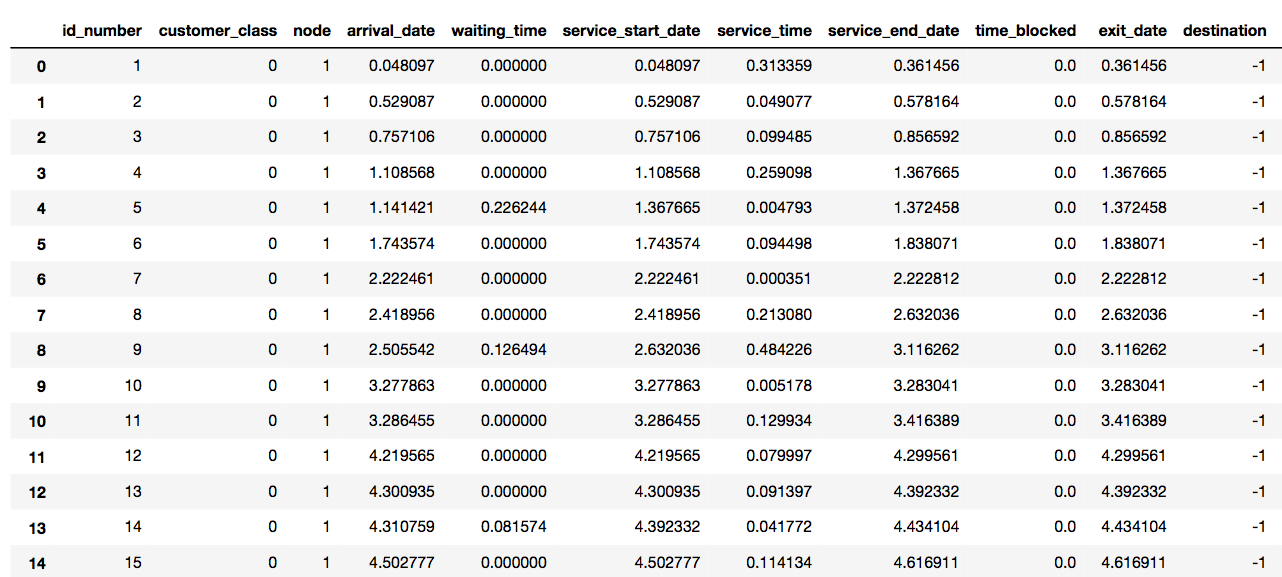
\includegraphics[width=\textwidth]{ciwrecords}
\end{frame}

\begin{frame}[fragile]
\begin{minted}[bgcolor=bgcol, fontsize=\scriptsize]{python}
N = ciw.create_network(
    Arrival_distributions={
        'Class 0': [['Exponential', 2.0], ['Exponential', 4.0]],
        'Class 1': [['Exponential', 2.0], ['Exponential', 3.0]]},
    Service_distributions={
        'Class 0': [['Deterministic', 0.5], ['Uniform', 0.2, 0.9]],
        'Class 1': [['Exponential', 2.0], ['Uniform', 0.3, 0.7]]},
    Transition_matrices={
        'Class 0': [[0.0, 0.0], [0.5, 0.0]],
        'Class 1': [[0.0, 0.2], [0.5, 0.1]]},
    Number_of_servers=[1, 2],
    Queue_capacities=[20, 'Inf'],
    Priority_classes={
        'Class 0': 1,
        'Class 1': 0},
    Class_change_matrices={
        'Node 1': [[0.0, 1.0], [0.0, 1.0]],
        'Node 2': [[0.8, 0.2], [0.0, 1.0]]}
)
\end{minted}
\end{frame}

\begin{frame}

\begin{center}
\textcolor{orange}{\url{https://github.com/CiwPython/Ciw}}
\end{center}

\vspace{8mm}

\begin{center}
\Large{\textcolor{darkorange}{\href{https://twitter.com/CiwPython}{@CiwPython}}}
\end{center}

\vspace{8mm}

\textbf{Ciw: An open source discrete event simulation library.}\\
\textit{Palmer GI, Knight VA, Harper PR, Hawa, AL.}
Under Review\\
PrePrint: \textcolor{darkorange}{\url{https://arxiv.org/abs/1710.03561}}
\end{frame}


\end{document}
